
\chapter{Data sources}

\pagestyle{fancy}

Not so long ago, all information used in a GIS had its origin in a paper map whose content was later transformed to adapt it to the particular nature of that GIS. Geographical data were obtained from the \textbf{digitalization} of printed cartography; that is, from the conversion of analogical maps into digital data that a GIS can handle.

Apart from the fact that we can use them in a GIS, digital data have many advantages and represent an important qualitative improvement. Digital data are easier to update, easier to distribute (specially since the Internet was created), use less physical space and are easier to maintain (digital data do not degrade. Their physical support does, but they are easy to replicate without losing their quality).

Techniques for geographical data acquisition have evolved, and it is possible now to create data that can be directly integrated into a GIS. Data sources that produce data ready for being used in a GIS are called \textbf{primary} data sources. Those that generate data that has to be adapted or converted are called \textbf{secondary} data sources.

In this chapter, we will see the main data sources that provide data for GIS.

\section{Remote sensing}

Remote sensing is the \textbf{acquisition of information about an object or phenomenon without making physical contact with it}. Instead of measuring the object itself, it measures the perturbations ---mainly the electromagnetic ones--- that it causes on its surroundings. In our case, it is applied to objects on the Earth's surface.

A remote sensing system contains the following elements (Figure \ref{Fig:Elements_remote_sensing}):

\begin{figure}[!hbt]   
\centering
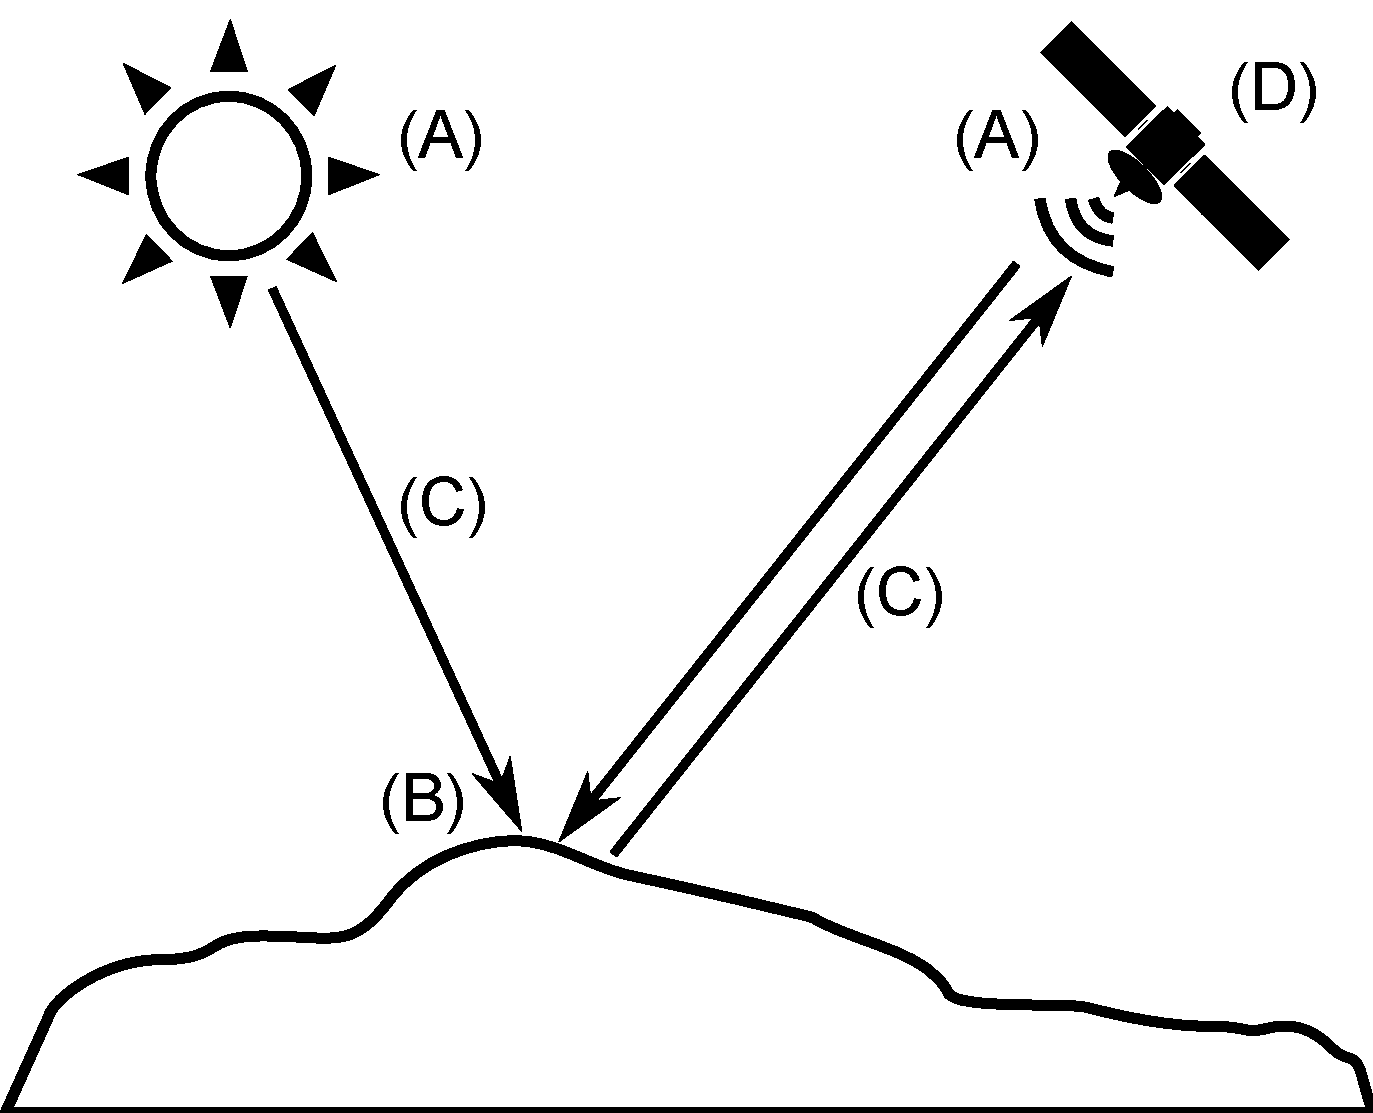
\includegraphics[width=.6\textwidth]{Data_sources/Elements_remote_sensing.pdf}
\caption{\small Elements in a remote sensing system.}
\label{Fig:Elements_remote_sensing} 
\end{figure}


\begin{itemize}
	\item \textbf{A source of radiation (A)}. It can be natural or artificial. Radiation emitted by the source reaches the Earth's surface and it is altered by the presence of the objects on that surface. Remote sensing studies that alteration. Objects themselves can emit radiation as well.
	\item \textbf{Objects (B) that interact with radiation} or can emit it, as mentioned above.
	\item \textbf{An atmosphere (C)} through which radiation moves from the source to the objects. The atmosphere also interacts with the radiation and alters it.
	\item \textbf{A receiver (D) which receives the radiation} once it has been emitted or altered by the objects. The receptor measures the intensity of the radiation coming from different points in the area being studied, and with them generates its final product (in most cases, and image). 
\end{itemize}

In this chapter, we will describe these elements in detail. To study the two first ones, we will also study some fundamentals about radiation and its interaction with matter. For describing the receivers that make part of a remote sensing system, we will separate them into two components: \textbf{sensors} and \textbf{platforms}.

Interaction with the atmosphere must be managed in order to eliminate its influence since, in most cases, we are interested in the object on the Earth's surface, not the atmosphere itself. Removing that influence is part of the post-processing of the data. Those processes are, however, rather complex, and they go beyond the scope of this book, so they will not be explained here.


\subsection{Electromagnetic radiation}

Electromagnetic radiation is caused by alterations in the electric and magnetic fields, which generate waves corresponding to each one of them. These waves move at the speed of light and can be described with the usual parameters such as wavelength and frequency. The range of frequencies (and corresponding wavelengths) of electromagnetic radiation is called the \textbf{electromagnetic spectrum}.

The spectrum is subdivided in regions depending on the wavelength, such as (from shorter to larger wavelength) gamma rays, X rays, ultraviolet region, visible region, infrared region or microwaves.


Radiation emitted by a radiation source is altered by the presence of objects that \textbf{absorb, transmit} or \textbf{reflect} it.

These three phenomena take place in a different proportion depending on the characteristics of the object and the radiation. For remote sensing, \textbf{the radiation that is reflected is the one of interest}, since it can be collected later and used to produce the data output.

Since each object reflects radiation at different wavelengths in a different way, this can be considered as a property of an object. The particular response of a given object and the way it alters a given radiation (which depends on its shape, material, etc.) is known as its \textbf{spectral signature} and can be used to identify the object.


\subsection{Sensors and platforms}

The two main technological elements in a remote sensing system, both of them related to the receiver, are the \textbf{sensor} and the \textbf{platform}.

The sensor is the element that can ``read'' the electromagnetic radiation and register its intensity for a given zone of the spectrum. It can be a simple photographic camera or a more specialized sensor.

\textbf{Passive} sensors use natural source of radiation (in most cases, sunlight), and just measure that radiation as it is reflected on the Earth's surface. \textbf{Active} sensors emit their own radiation, and then collect it back after it has been reflected. Here is a simple example to better understand this: a photographic camera is a passive sensor, while a photographic camera that uses a flash unit is an active one. The radiation emitted by an active sensor does not have to be visible light (as in the case of the flash); the sensor can emit in other regions of the spectrum.

Technologies such as \textbf{radar} or \textbf{LiDAR} (similar to radar but with light pulses instead of radio waves) are based on active sensors.

The sensor is \textbf{mounted on a platform}, and it performs its data acquisition from it. \textbf{Several sensors} can be mounted on a single platform.

The two main types of platforms are those located inside the Earth's atmosphere (mostly on airplanes) and those outside of it (on satellites).

The advantage of airplanes is their \textbf{availability}, since they can be piloted and used to cover any place on earth at any moment. Satellites, on the other hand, cannot be guided, and its movement is fixed and defined by a set of parameters known as \textbf{orbital parameters}, which define the orbit described by the satellite around the Earth.

Orbits can be classified according to their \textbf{rotation axis} or their \textbf{movement}. Two particular cases are the \textbf{geosynchronous} orbits (the satellite is located in a fixed point and its movement follows the earth rotation) and the \textbf{heliosynchronous} (the satellite passes over any given point in its path always at the same local solar time).
	
\subsubsection{Resolutions}

The the most important parameters that define the characteristics of a remote sensing system are its \textbf{resolutions}. These define the level of detail of the products that it creates. Resolutions depend on both the sensor and the platform as an single operative unit, and on the individual characteristics of each of them. Four resolutions can be defined:

\begin{itemize}
	\item \textbf{Spatial resolution}. It indicates the size of the smaller object that can be distinguished. If the output is an image, the spatial resolution is the real size of the area represented by a single pixel.
	\item \textbf{Spectral resolution}. It indicates the amplitude of each of the regions of the spectrum that is registered. It is defined by the total amplitude that is covered and the number of sections into which it is divided. The measurement corresponding to each of these sections will usually be stored in a separate band in the resulting image. 
	\item \textbf{Radiometric resolution}. It indicates the level of detail of the intensity measurement taken for each of the spectral regions that are registered. 
	\item \textbf{Temporal resolution}. It indicates the time that it takes the sensor to return to a given place. It makes sense only for orbital sensors. It depends on the platform characteristics, such as its attitude, and also on the sensor characteristics.
\end{itemize}

It is not possible (for technical and theoretical reasons) to have a sensor in which all the above resolutions are maximized simultaneously. Some sensors might favor certain resolutions, while others might favor a different one.

When using images coming from remote sensing in a GIS, we should consider which resolution is more important (for instance, to locate elements that have a small size, high spatial resolution is needed). Using data from several different sensors is a good strategy for overcoming these limitations.


\subsection{Photogrammetry}

Photogrammetry is the technique used to study and precisely define the shape, size and position in space of any object, using measurements taken on one or several photographs. Of special interest to GIS is the branch of photogrammetry known as \textbf{aerial photogrammetry}, which uses aerial photographs and it is mainly used for generating elevation data through a process known as \textbf{restitution}.

Instead of single images, the branch of photogrammetry known as \textbf{stereophotogrammetry} uses pairs of images, each of them taken from a different point. These images form a \textbf{stereo pair} and with them a three-dimensional reconstruction of the original scene can be produced. This can be used by an operator to ``see'' the scene with \textbf{depth and volume}, so that terrain forms can be identified and elevation information obtained. 

If using satellite images, stereo pairs can be obtained from those platforms and sensors that allow \textbf{changing the angle of vision}, so in the same satellite pass pictures of a given area can be taken from different points.

Photogrammetry can be \textbf{analogical} or \textbf{digital}, the latter being the one more related to the field of GIS.

Stereoplotters are used to combine and align the images that form the stereo pair. Current stereoplotters are called \emph{analytical stereoplotters}, and contain elements from GIS, along with more specific elements. Among these, we find specific visualization software and peripherals such as 3D mouses or other mechanical elements found in analogical photogrammetric devices, making it easy for operators to adapt to this new type of tools.

\section{Printed cartography. Digization}

A large amount of cartography exists in printed form, such as maps or old analogical aerial photographs. To be used in a GIS, this cartography has to be \textbf{digitized}. That means creating raster or vector layers from them. In this latter case it also implies \textbf{separating the different types of information} that the map might contain, since the information in a single printed map would be stored in independent layers, in GIS

Digitizing a printed cartographic document involves three steps: 

\begin{itemize}
\item \textbf{Georeferencing} the original document. That is, setting a geographical context (coordinate system, control points, etc.), so the digitized element that we will produce are correctly referenced.
\item \textbf{Digitizing the spatial component}. That is, creating the corresponding geometries.
\item \textbf{Digitizing the thematic component}. Creating cell values for raster layers or attributes in the case of vector ones.
\end{itemize}

Digitization can be \textbf{manual} or \textbf{automatic}. In the first case, an operator introduces the value, while in the second one that is done by an algorithm.

To create raster layers, the most common method is to \textbf{scan} the original document using a \textbf{scanner}, which creates a digital image from an analogical one.

High-end scanners specifically designed for working with cartographic documents are available. Generic scanners, however, can be used for this task with acceptable result in terms of accuracy and distortion. 

Two parameters define the characteristics of a scanner: its \textbf{spatial resolution} and its \textbf{radiometric resolution}. The first one is usually measured in \textbf{dots per inch} (DPI) and indicates the number of points (cells) that the sensor will create in the resulting image for each length unit in the original document. Radiometric resolution defines the ability of the sensor to separate between two different colors.

The ideas discussed in chapter \ref{Fundamentals} about scale should be taken into account here as well. Working with a higher resolution (if the scanner allows it) will not always mean adding more information to the resulting image, since it might not exist in the original document. We would just have a volume of data larger than the one needed to capture all the information in the printed document, but not more information.

In the case of vector layers, \textbf{manual digitization} is the most common method. An operator defines the features, tracing its geometries and entering the associated attribute data.

To digitize geometries, the operator can use the \textbf{editing functionality of a GIS} and work on the screen of the computer using its mouse as tracing device, or use specialized peripherals such as a \textbf{digitizing tablet}. In the first case, digitizing takes places on the screen, so a digital version of the printed document is needed (although not a vector one), which can be obtained by scanning it. The full digitization process involves two steps which include two different types of digitization: from printed map to raster image (automatic), and from image to vector features (manual). If using a tablet, the printed map can be used directly to trace geometries on it.

Automatic digitization of geometries in a vector layer is known as \textbf{vectorization}. A digital image is needed, so the original document has to be scanned first. The vectorization algorithm analyzes the map and finds the elements that it contains, creating the corresponding vector layer elements from that. Manual work is usually needed to complete and correct the resulting data, since this tends to be a complex and error-prone process in which data preparation has a great importance, and a fully automatic alternative is not possible most of the time.

A particular case of digitization is the \textbf{creation of layers from a set of values representing some spatial process}. That is, when the original analogical document is not a map, but just a set of values. This process is known as \textbf{geocoding}, and it involves assigning coordinates to those values, and then creating the corresponding layers with the combination of the original thematic data and the geographical information (the spatial component) that resulted from the geocoding process.

The original alphanumeric data can be introduced manually or using an automated approach, such as scanning the document and then using some character recognition (OCR) software.

A particular and very popular case of geocoding (although in this case the document is not analogical) is \textbf{geotagging}, in which coordinates are assigned to digital images.


\subsection{Digitization Quality}

One of the most important aspects of digitization is the \textbf{quality of its result}, which should be as close as possible to the quality of the document being digitized. Digitization is never perfect, regardless of the accuracy of the equipment that is used or the skills of the person that performs it. There will always be errors and deficiencies.

Along with the errors introduced in the different phases of the digitization process, the original source documents might contain their own errors as well. For instance, scanning a map might introduce errors due to geometric distortions, but that map might contain itself some distorsion due to its previous use.

Information contained in a cartographic document might include elements that are problematic and will decrease the quality of the resulting data. A map that contains stains or has some lines that are not correctly visible will result in errors when digitizing its vector features (specially in the case of automatic digitization) regardless of the quality of the scanning process that is required before. 
 
Among the errors due to the digitization process itself, and not related to the document characteristics, \textbf{mismatching nodes in vector geometries} are one the most common problems (Figure \ref{Fig:Errors_digitization})

\begin{figure}[!hbt]   
\centering
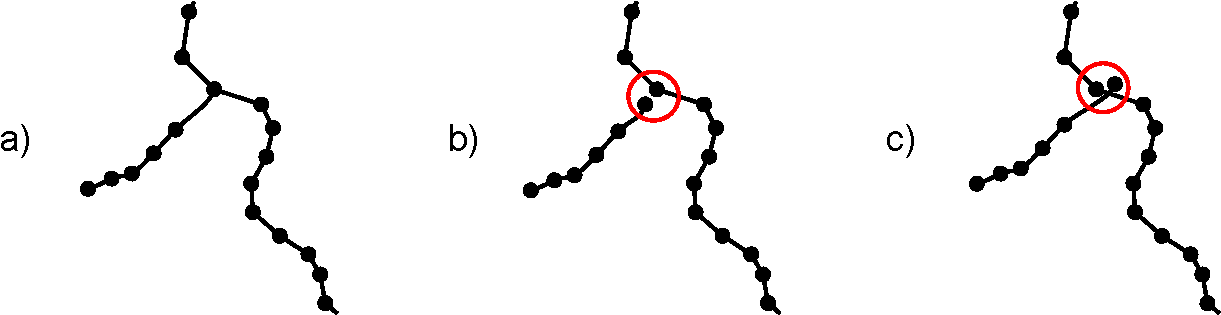
\includegraphics[width=\textwidth]{Data_sources/Errors_digitization.pdf}
\caption{\small Digitization errors. a) Correct version with matching nodes. b) and c) Incorrect versions, with mismatching nodes, causing wrong disconnected lines.}
\label{Fig:Errors_digitization} 
\end{figure}


For this reason, the editing capabilities of GIS include additional functionalities to avoid these errors while digitizing, helping the user and allowing an accuracy and quality that would not be possible without such aids. Among them, the automatic adjustment of geometry nodes based on predefined tolerances (known as \textbf{snapping}) is specially relevant, since it can guarantee a correct relation between the nodes of different geometries (belonging or not to the same feature)

This is particularly important in the case of digitizing not only the geometries, but also the \textbf{topological information} that is contained in the original document (such as the connection between the roads in a map sheet).  Also, when digitizing geometries and their topology, certain additional rules must be followed, such as only digitizing the shared sides of adjacent polygons once. Additional information must also be digitized, such as the definition of nodes when lines cross each other and there is a relation between the objects they represent (for instance, a crossing between two road lines that represents a point where vehicles can pass from one road to the other).

\section{GPS}

One of the most relevant advancements in geographical data sources have been \textbf{global navigation satellite systems} (GNSS). These systems allow, \textbf{for any given point and at any time, to know the exact location of that point} with an accuracy of a few meters or less. To do it, they use a constellation of satellites to which information is transmitted from the study point, and use that transmission to compute the coordinates at which the point is located.

The first and most popular of these systems is the \textbf{Global Positioning System} (GPS). It has 24 active satellites (the satellite segment), along with terrestrial stations to control them (the control segment), and it is based on \textbf{trilateration}. Distances are measured from a GPS unit (the user segment) to a certain number of satellites. Knowing those distances and the exact position of the satellites, the position of the unit can be computed. Position is computed with its \emph{x, y} and \emph{z} coordinates. The GPS system uses WGS-84 as its reference ellipsoid.

The satellite network is designed to guarantee that, from any point of the Earth's surface, and at any time, a GPS unit can locate the required number of satellites to compute its position.

There are \textbf{several error sources} that might affect the accuracy of the position computed by a GPS unit. Among them, we find errors in the position of satellites, errors due to the effect of the Earth's atmosphere on the GPS signal, and also those caused by the accuracy problems of the clocks used to measure signal travel time (which is then converted into travel distance). \textbf{Selective availability} was a random error introduced in the GPS signal with military purposes. It was, however, removed on May 2, 2000.

Among the techniques use to correct or minimize these errors, \textbf{differential GPS} is the most important one. It was originally conceived to remove the effect of selective availability, but can be used to correct a large part of the other errors that affect the GPS system.

To apply differential GPS, along with the receiver unit for which its position is to be computed, a \textbf{second receiver} is needed. It has to be a \textbf{fixed} one, not mobile, and its coordinates have to be known with great precision. This receiver is, itself, a high-precision unit, and broadcasts information that other units can use to correct their position. 

The idea is that errors that affect the mobile GPS unit \textbf{also affect the fixed reference one}. The error for the reference unit can be computed, since its position is known, and using the discrepancy between that real position and the one computed using the GPS system, the position of other GPS units can be corrected.

Using this differential correction, a regular GPS can obtain coordinates with an accuracy of around 2 meters in their $x$ and $y$ components, and around 3 meters in the $z$ component. Without differential GPS, an accuracy of just 10--20 meters is to be expected.

Precision of the GPS system depends on the GPS unit. There are many classes of GPS receivers, but the main ones, from the point of view of GIS, are two:

\begin{itemize}
	\item \textbf{GPS for general use}. This units are low-cost \textbf{small and portable} ones, for outdoors activities, where a high accuracy is not required. The GPS receivers that are found in smartphones also fall in this category.
	\item \textbf{GPS for surveying}. Larger units, usually with independent antennas that are connected to the receiver to increase accuracy. It also ensures better location of satellites in difficult conditions, such as under forest canopy. They are designed for professional use.
\end{itemize}	


Regarding its connection with GIS, GPS units can collect coordinates and then create GIS layers with them. They can store points (called \textbf{waypoints} in the usual GPS terminology), or capture the path followed by the user (called a \textbf{track}). In this last case, the receiver stores points at regular intervals, so the user can just move and does not have to manually store the coordinates along the route. This information can be later introduced in a GIS for further analysis or visualization. 


\section{Voluntary Geographical Information}

The participative ideas of the so-called \textbf{Web 2.0}, when combined with tools such as recreational GPS units, or with simplified software for editing and digitizing, result in interesting initiatives in which ordinary people, with no specific training in cartography or surveying, can acquire and share geographical information. 

Although this cannot be considered a different data source (the techniques and devices used have already been described in previous sections), there is an important change in the philosophy behind data collection and usage, which makes it worth to treat this type of data separately in the context of this book.

The term \textbf{Volunteered Geographical Information} (VGI) refers to the use of the Internet to create, manage, and share geographical information which has been voluntarily contributed by a community of users, using the Internet as well. The set of techniques and tools used by those users is termed \textbf{neogeography}. 

Neogeography has changed some fundamental ideas in cartography, since it has modified the traditional concept of geographical information (which was just created by a very skilled few), its characteristics, or the role it played on certain fields. The following are some ideas about these changes and neogeography itself.


\begin{itemize}
	\item \textbf{Popularization and democratization}. Cartographic production has always been in the hands of governments or agencies, and in many cases has been strongly censored due to its high strategical value. With the advent of VGI, geographical information becomes more democratic, and its creation is a free, participative and unrestricted process. The ``top-down'' approach that had dominated the production and use of cartography gets inverted.
	\item Citizens become \textbf{sensors} and have more conscience of their geospatial reality.
	\item Cartographic production loses its ``Mysticism''.	
\end{itemize}

The most relevant VGI project nowadays is \textbf{OpenStreetMap} (OSM), a `` collaborative project to create a free editable map of the world.''.


\section{Metadata}

Regardless of their origin, data might need additional data to be interpreted. For instance, if we have the coordinates of a point, to correctly interpret it we need, among other things, the coordinate system in which those coordinates are expressed. The data we work with (the coordinates), should be accompanied by some ancillary data (such as the EPSG code of the coordinate system).

This ancillary data are known as \textbf{metadata}. Metadata are \textbf{data about the data}, and their purpose is to \textbf{explain the meaning of the data}. That is, they help the user to better understand the meaning of the data and the information that they contain. Metadata are an additional document that accompanies the data, and that allows a better management and use of them.

Within a GIS, metadata are usually \textbf{associated to a layer and its content}, and can be \textbf{referred to both components} (spatial and thematic).

The concept of metadata is not something exclusive of digital geographical data. A printed map has metadata in a certain way. A legend or a text in its margin with information about the date in which it was created are also metadata. In the case of digital metadata, the metadata is \textbf{independent from the data itself}. That allows us to perform operations \textbf{separately on the metadata}, which opens many possibilities and gives them a great value.

Two of the main functions of metadata are \textbf{ensuring the correct use of data} and \textbf{facilitating its management, discovery and exploitation}.

Geographical data, as many other types of data, are usually created for a given purpose, and that purpose does not have to be contained in the data themselves or be easy to infer from them. When those are used for a different purpose, problems might arise, since data might have some deficiencies when used in this new context. With the help of metadata, this can be solved. They might help, for instance, to \textbf{avoid the use of outdated datasets or datasets with insufficient accuracy}. Knowing the parameters that define a dataset (original scale, date, etc.), we can better judge whether or not to use them for a given task.

Data creators must take care of \textbf{adding enough metadata to them}, and users must \textbf{consult their associated metadata} before using any data.

Regarding data management, metadata facilitate operations such as searching data in larger datasets or data collections. Metadata can contain a ``summary'' of the full data they accompany, and that can be used to \textbf{make search operations more efficient} if they use a geographical criteria. For instance, if a user wants to find whether a data collection has some data for a given area, the full content of each vector layers in the collection should be checked, to see if any of its geometries falls within the requested region. This can be a lengthy operation. If each layer has an associated metadata with its extent, the query can be executed with the metadata, which is much faster, as it is independent of the number of features in the layer. This is fundamental when creating \textbf{data catalogs}, which respond to user queries based on the information contained in the metadata.


\subsection{Content of metadata. Metadata creation}

The information contained in the metadata associated to geographical data depends on parameters such as the \textbf{representation model} used, the \textbf{format} in which data are stored (file format, database, etc.), the \textbf{organization, entity or individual responsible} of the data or the \textbf{element they are associated to} (set of layers, layer, feature, etc.).

Some of the common elements that are added to metadata in the case of geographical data are \textbf{identification} information (to identify them in a unique way and distinguish the from other data), information about their quality (including their origin, and the origin of the data they might derive from ---the \textbf{data lineage}---) or information about its distribution (access, license, etc.).
 
Metadata can be created \textbf{at the data origin}, just at the same time as the data themselves are created. It can also be \textbf{extended later} by data distributors, managers or users.

Most of the metadata content is created manually, and there are specific applications for that, sometimes connected to desktop GIS tools. Metadata elements that can be extracted from the data itself (such as the data extent), can be created automatically.

Metadata are generally stored as \textbf{additional files} that accompany the data files, or they are stored \textbf{as part of a database}.


\pagestyle{empty}
